\documentclass[journal,12pt,twocolumn]{IEEEtran}
%
\usepackage{setspace}
\usepackage{gensymb}
%\doublespacing
\singlespacing

\usepackage[cmex10]{amsmath}
\usepackage{amsthm}
%\usepackage{iithtlc}
\usepackage{mathrsfs}
\usepackage{txfonts}
\usepackage{stfloats}
\usepackage{bm}
\usepackage{cite}
\usepackage{cases}
\usepackage{subfig}
%\usepackage{xtab}
\usepackage{longtable}
\usepackage{multirow}
%\usepackage{algorithm}
%\usepackage{algpseudocode}
\usepackage{enumitem}
\usepackage{mathtools}
\usepackage{steinmetz}
\usepackage{tikz}
\usepackage{circuitikz}
\usepackage{verbatim}
\usepackage{tfrupee}
\usepackage[breaklinks=true]{hyperref}
%\usepackage{stmaryrd}
\usepackage{tkz-euclide} % loads  TikZ and tkz-base
%\usetkzobj{all}
\usetikzlibrary{calc,math}
\usepackage{listings}
    \usepackage{color}                                            %%
    \usepackage{array}                                            %%
    \usepackage{longtable}                                        %%
    \usepackage{calc}                                             %%
    \usepackage{multirow}                                         %%
    \usepackage{hhline}                                           %%
    \usepackage{ifthen}                                           %%
  %optionally (for landscape tables embedded in another document): %%
    \usepackage{lscape}     
\usepackage{multicol}
\usepackage{chngcntr}
%\usepackage{enumerate}

%\usepackage{wasysym}
%\newcounter{MYtempeqncnt}
\DeclareMathOperator*{\Res}{Res}
%\renewcommand{\baselinestretch}{2}
\renewcommand\thesection{\arabic{section}}
\renewcommand\thesubsection{\thesection.\arabic{subsection}}
\renewcommand\thesubsubsection{\thesubsection.\arabic{subsubsection}}

\renewcommand\thesectiondis{\arabic{section}}
\renewcommand\thesubsectiondis{\thesectiondis.\arabic{subsection}}
\renewcommand\thesubsubsectiondis{\thesubsectiondis.\arabic{subsubsection}}

% correct bad hyphenation here
\hyphenation{op-tical net-works semi-conduc-tor}
\def\inputGnumericTable{}                                 %%

\lstset{
%language=C,
frame=single, 
breaklines=true,
columns=fullflexible
}
\newenvironment{amatrix}[1]{%
  \left(\begin{array}{@{}*{#1}{c}|c@{}}
}{%
  \end{array}\right)
}
\DeclarePairedDelimiter\abs{\lvert}{\rvert}%
\DeclarePairedDelimiter\norm{\lVert}{\rVert}%

% Swap the definition of \abs* and \norm*, so that \abs
% and \norm resizes the size of the brackets, and the 
% starred version does not.
\makeatletter
\let\oldabs\abs
\def\abs{\@ifstar{\oldabs}{\oldabs*}}
%
\let\oldnorm\norm
\def\norm{\@ifstar{\oldnorm}{\oldnorm*}}
\makeatother

\newtheorem{theorem}{Theorem}[section]
\newtheorem{problem}{Problem}
\newtheorem{proposition}{Proposition}[section]
\newtheorem{lemma}{Lemma}[section]
\newtheorem{corollary}[theorem]{Corollary}
\newtheorem{example}{Example}[section]
\newtheorem{definition}[problem]{Definition}
%\newtheorem{thm}{Theorem}[section] 
%\newtheorem{defn}[thm]{Definition}
%\newtheorem{algorithm}{Algorithm}[section]
%\newtheorem{cor}{Corollary}
\newcommand{\BEQA}{\begin{eqnarray}}
\newcommand{\EEQA}{\end{eqnarray}}
\newcommand{\define}{\stackrel{\triangle}{=}}
\bibliographystyle{IEEEtran}
%\bibliographystyle{ieeetr}
\providecommand{\mbf}{\mathbf}
\providecommand{\pr}[1]{\ensuremath{\Pr\left(#1\right)}}
\providecommand{\qfunc}[1]{\ensuremath{Q\left(#1\right)}}
\providecommand{\sbrak}[1]{\ensuremath{{}\left[#1\right]}}
\providecommand{\lsbrak}[1]{\ensuremath{{}\left[#1\right.}}
\providecommand{\rsbrak}[1]{\ensuremath{{}\left.#1\right]}}
\providecommand{\brak}[1]{\ensuremath{\left(#1\right)}}
\providecommand{\lbrak}[1]{\ensuremath{\left(#1\right.}}
\providecommand{\rbrak}[1]{\ensuremath{\left.#1\right)}}
\providecommand{\cbrak}[1]{\ensuremath{\left\{#1\right\}}}
\providecommand{\lcbrak}[1]{\ensuremath{\left\{#1\right.}}
\providecommand{\rcbrak}[1]{\ensuremath{\left.#1\right\}}}

\providecommand{\system}{\overset{\mathcal{H}}{ \longleftrightarrow}}
	%\newcommand{\solution}[2]{\textbf{Solution:}{#1}}
\newcommand{\solution}{\noindent \textbf{Solution: }}
\newcommand{\cosec}{\,\text{cosec}\,}
\providecommand{\dec}[2]{\ensuremath{\overset{#1}{\underset{#2}{\gtrless}}}}
\newcommand{\myvec}[1]{\ensuremath{\begin{pmatrix}#1\end{pmatrix}}}
\newcommand{\mydet}[1]{\ensuremath{\begin{vmatrix}#1\end{vmatrix}}}
%\numberwithin{equation}{section}
\numberwithin{equation}{subsection}
%\numberwithin{problem}{section}
%\numberwithin{definition}{section}
\makeatletter
\@addtoreset{figure}{problem}
\makeatother
\let\StandardTheFigure\thefigure
\let\vec\mathbf
\usepackage{mathtools, nccmath}

\begin{document}

\begin{center}
\huge Assignment 4\\

\large Shaik Zeeshan Ali\\
\large AI20MTECH11001\\
\end{center}
\begin{abstract}
This document is about isosceles triangles having a common base.
\end{abstract}
Download all python codes from 
\begin{lstlisting}
https://github.com/Zeeshan-IITH/IITH-EE5609/new/master/codes
\end{lstlisting}

and latex-tikz codes from 
\begin{lstlisting}
https://github.com/Zeeshan-IITH/IITH-EE5609
\end{lstlisting}
\section{problem}
$\triangle ABC$ and $\triangle DBC$ are two isosceles triangles on the same base $BC$.Prove that $\angle ABD=\angle ACD$.
\section{construction}
In an Isosceles triangle the angles opposite to sides of equal length are equal.Therefore the angles $\angle ABC=\angle ACB$ and $\angle DBC=\angle DCB$.Let the vertex $B$ be at origin and not lose generality.Since the two triangles are isosceles,$\norm{\vec{B}-\vec{D}}=\norm{\vec{C}-\vec{D}}$ and $\norm{\vec{A}-\vec{B}}=\norm{\vec{A}-\vec{C}}$.
\section{Explanation}
The triangles $\triangle ABC$ and $\triangle DBC$ are isosceles triangles,so
\begin{align}
    \norm{\vec{A}-\vec{B}} = \norm{\vec{A}-\vec{C}}\label{eq:1}\\
    \norm{\vec{D}-\vec{B}} = \norm{\vec{D}-\vec{C}}\label{eq:2}
\end{align}
From equation \eqref{eq:1},we get
\begin{multline}
    {\brak{\vec{A}-\vec{B}}^T\brak{\vec{A}-\vec{B}}}={\brak{\vec{A}-\vec{C}}^T\brak{\vec{A}-\vec{C}}}\\
    {\brak{\vec{A}-\vec{B}}^T\brak{\vec{A}-\vec{D}+\vec{D}-\vec{B}}}=\\{\brak{\vec{A}-\vec{C}}^T\brak{\vec{A}-\vec{D}+\vec{D}-\vec{C}}}\\
    {\brak{\vec{A}-\vec{B}}^T\brak{\vec{D}-\vec{B}}}=\\
    {\brak{\vec{A}-\vec{C}}^T\brak{\vec{D}-\vec{C}}
    +\brak{\vec{B}-\vec{C}}^T\brak{\vec{A}-\vec{D}}}\label{eq:3}
\end{multline}
Doing the below calculation,we get
\begin{multline}
    {\brak{\vec{C}-\vec{B}}^T\brak{\vec{A}-\vec{B}}-\brak{\vec{C}-\vec{B}}^T\brak{\vec{D}-\vec{B}}}=\\
    {\brak{\vec{A}-\vec{C}}^T\brak{\vec{B}-\vec{C}}-\brak{\vec{D}-\vec{C}}^T\brak{\vec{B}-\vec{C}}}\\
    {\brak{\vec{C}-\vec{B}}^T\brak{\vec{A}-\vec{D}}}={\brak{\vec{A}-\vec{D}}^T\brak{\vec{B}-\vec{C}}}\label{eq:6}
\end{multline}
\begin{figure}[!h]
    \centering
    \resizebox{\columnwidth}{!}{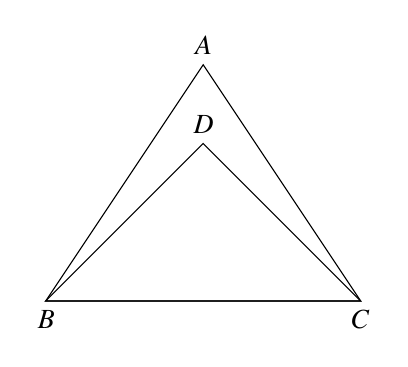
\begin{tikzpicture}
    \coordinate (B) at (0,0);
    \coordinate (A) at (2,3);
    \coordinate (C) at (4,0);
    \coordinate (D) at (2,2);
    \draw (A)node[above]{$A$}--(B)node[below]{$B$}--(C)node[below]{$C$}--cycle;
    \draw (D)node[above]{$D$}--(B)node[]{}--(C)node[]{}--cycle;
\end{tikzpicture}
}
    \caption{Isosceles triangles with common base BC}
    \label{myfig:1}
\end{figure}
Since $\brak{\vec{A}-\vec{D}}^T\brak{\vec{B}-\vec{C}}$=${\brak{\vec{B}-\vec{C}}^T\brak{\vec{A}-\vec{D}}}$, the equation \eqref{eq:6} can be written as
\begin{align}
    {\brak{\vec{B}-\vec{C}}^T\brak{\vec{A}-\vec{D}}}&={\brak{\vec{C}-\vec{B}}^T\brak{\vec{A}-\vec{D}}}\\
    {\brak{\vec{B}-\vec{C}}^T\brak{\vec{A}-\vec{D}}}&=-{\brak{\vec{B}-\vec{C}}^T\brak{\vec{A}-\vec{D}}}\\
    2{\brak{\vec{B}-\vec{C}}^T\brak{\vec{A}-\vec{D}}}&=0\\
    \brak{\vec{B}-\vec{C}}^T\brak{\vec{A}-\vec{D}}&=0\label{eq:7}
\end{align}
Taking the inner product of $A-B,B-D$ and $A-C,D-C$,we get
\begin{align}
    \cos\angle ABD=\frac{\brak{\vec{A}-\vec{B}}^T\brak{\vec{D}-\vec{B}}}{\norm{\vec{A}-\vec{B}}\norm{\vec{D}-\vec{B}}}\\
    \cos\angle ACD=\frac{\brak{\vec{A}-\vec{C}}^T\brak{\vec{D}-\vec{C}}}{\norm{\vec{A}-\vec{C}}\norm{\vec{D}-\vec{C}}}
\end{align}
Subtracting the above equations we get 
\begin{align}
    \cos\angle ABD-\cos\angle ACD\\
    =\frac{\brak{\vec{A}-\vec{B}}^T\brak{\vec{D}-\vec{B}}-\brak{\vec{A}-\vec{C}}^T\brak{\vec{D}-\vec{C}}}{\norm{\vec{A}-\vec{C}}\norm{\vec{D}-\vec{C}}}\\
    =\frac{\brak{\vec{B}-\vec{C}}^T\brak{\vec{A}-\vec{D}}}{\norm{\vec{A}-\vec{C}}\norm{\vec{D}-\vec{C}}}\\
    \intertext{Using the equation \eqref{eq:7},we get}
    \cos\angle ABD-\cos\angle ACD=0\\
    \cos\angle ABD=\cos\angle ACD\\
    \angle ABD=\angle ACD
\end{align}
\end{document}
